\section{Introduction}

% \begin{it}
% The key point to reach by the end of the introduction is a clear statement of what the specific research question that you investigated in the project, and what it was the motivated this question. Typically this is done by first setting the scene with a description of the general subject area as a whole.  Then you would highlight key scientific developments that make the question you have investigated (i) relevant and (ii) lacking an answer.

% It is common for introductions to end with a brief sketch of the main content of the rest of the report; there is no harm in summarising the conclusion, as this can help the reader pace themselves as they work through your report.
% \end{it}

\hl{Intro to knot theory/ applications in physics/ need for knot invariant and classification -> lead onto the general idea of a classification problem : ML is known to be well suited to this}

Knot theory is the study of knots: self-entangled, closed loops in $\mathbb{R}^{3}$. It doesn't take too much searching to discover the ubiquity of these such knots, stretching from the super-coiling nature of DNA \cite{bauer1980supercoiled} to forms of the path integral in a topological quantum field theory \cite{witten1994quantum}. The abundance of knots in such physical systems highlights the importance of knot theory and its study in physics.

The search for a unique, invariant property of knots has eluded mathematicians and physicists since the foundations of knot theory in the $19^{th}$ century. In searching for such a property, academics have unveiled a plethora of methods that categorize and distinguish knots to increasing levels of complexity (i.e.\ number of crossings) - however, each of these methods falls short in one way or another, unable to distinguish between every (known) knot uniquely (see figure \ref{fig:knot_comp}). And so the search is still on to discover a new and complete knot invariant. 

\begin{figure}[h]%
    \centering
    \subfloat[\centering Conway knot]{{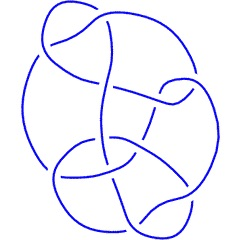
\includegraphics[width=5cm]{Images/Conway knot.jpeg}}}
    \qquad
    \subfloat[\centering Unknot]{{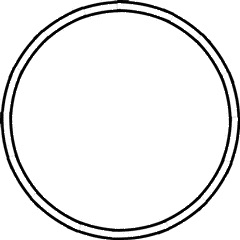
\includegraphics[width=5cm]{Images/unknot.jpeg}}}%
    \caption{The Conway knot (a), an 11 crossing knot, shares the same Alexander-Conway polynomial as the unknot (b).}%
    \label{knot_comp}%
\end{figure}

This is a classification problem; finding a way to distinguish between each \emph{class} of knots (unknot, Conway knot...) given specific \emph{features} (Alexander-Conway polynomial, DT code, XYZ position...).

Machine learning methods make use of algorithmic frameworks to probabilistically determine a mapping function (f) given a set of input features ($\vec{X}$) and their corresponding output (y). Through this, machine learning methods provide solutions to classification problems, and so we seek to apply these methods to investigate the classification of knots.

Building on prior work by Sleiman et.\ al.\ \cite{sleiman2022geometric} in which it was successfully found that the segment-to-segment writhe of a knot resulted in near perfect ($\approx99\%$) classification \footnote{up to 10 crossings}, we ask ourselves if this result is consistent when trained in an unsupervised environment, one in which the machine learning model is not given the labels of the corresponding data. Ultimately we want to find if the machine learning model is able to identify its own labels and classify its data unprompted. As a result, the model would be able to distinguish between knots, generate a latent space with discrete mapping of the different types of knots and additionally, generate new knots based on it's learned parameters (specifically knots on which the model was not trained). 
In doing so, we learn more about the underlying mathematical mechanism by which segment-to-segment writhe leads to classification of knots and seek to understand the repercussions of this from a physics point of view.

This report will tackle how this was completed and the results found. 
However first, a background on knot theory, machine learning and generative machine learning will be presented to give the reader sufficient context for the discussions that follow.


\hl{Road map:}

    1. Fundamentals:
   - ML Fundamentals: Basics of machine learning. 
   Supervised and unsupervised learning, neural networks, and the fundamentals of how models learn from data.

   - Generative Models: Generative Adversarial Networks (GANs) and Variational Autoencoders (VAEs).

   - Knot Theory Basics: Review the fundamental concepts of knot theory. Understand the different types of knots, their properties, and how they can be represented.

    2. Literature Review:
   - Relevant Research Papers: Machine learning and knot theory. 
   Importantly -> note: state-of-the-art techniques, challenges, and gaps in the existing literature.

   - Explore Applications: Investigate how generative machine learning has been applied in other mathematical and physical domains -> any insights or methodologies that can be adapted to knot theory?

    3. Specific Problem or Question:
   - Define Scope: Narrow down focus within the intersection of generative machine learning and knot theory.

   - Identify Challenges: Challenges that arise in applying generative machine learning to knot theory. This could include issues related to data representation, model complexity, or interpretability.

    4. Data Collection and Preparation:
   - Data Availability: Use of existing dataset.

   - Data Preprocessing: Clean and preprocess data to ensure it's suitable for training machine learning models. This may involve normalizing, scaling, or transforming your knot data (should already be done).

    5. Experimentation and Model Development:
   - Pytorch.

   - Model Architecture: Design generative model architecture.

   - Training and Evaluation: Train model using appropriate algorithms and evaluate performance. Iterate on model based on the results.

    6. Interpretation and Analysis:
   - Interpret Results: Analyze results of experiments. Evaluate generative models ability to produce \emph{meaningful} instances of knots.

   - Implications: Implications of findings on knot theory. How can generative machine learning contribute to the understanding or discovery of new aspects of knots.

   7. Conclusions:
   - Future Work: Directions for future research in the intersection of generative machine learning and knot theory.

